\documentclass[11pt]{article}
\pdfinfoomitdate=1\pdftrailerid{}
\usepackage[letterpaper,margin=.7in,headheight=15pt,headsep=18pt,footskip=24pt]{geometry}
\usepackage[T1]{fontenc}\usepackage{lmodern,amsmath,amssymb,array,booktabs,fancyhdr,tikz,pifont}
\usepackage{enumitem}\setlist{nosep}
\renewcommand{\familydefault}{\sfdefault}\setlength{\parindent}{0pt}\setlength{\parskip}{5pt}
\definecolor{cred}{RGB}{214,39,40}\definecolor{cblue}{RGB}{31,92,204}
\pagestyle{fancy}\fancyhf{}\renewcommand{\headrulewidth}{0pt}
\fancyhead[L]{\small Week NN / Patterns you cannot avoid / Facilitator guide}
\fancyfoot[L]{\scriptsize Bellingham Math Circle / Week NN / NN-FAC-v1}\fancyfoot[R]{\thepage}
\usepackage{needspace}
\newcommand{\head}[1]{\par\needspace{8\baselineskip}\medskip\textbf{\large #1}\par}
\newcommand{\sub}[1]{\par\needspace{4\baselineskip}\textbf{#1}\par}
\newcommand{\st}[1]{\texttt{#1}}
% generated by figs.py
\newcommand{\launchfig}{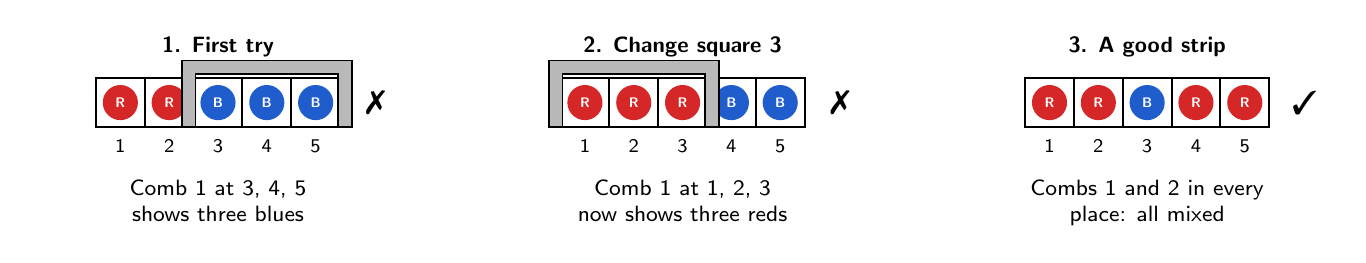
\begin{tikzpicture}\draw[line width=0.7pt] (0.000,0.000) rectangle (0.620,0.620);
\node[font=\scriptsize, anchor=base] at (0.310,-0.320) {1};
\fill[cred] (0.310,0.310) circle (0.223);\node[text=white,font=\bfseries\tiny] at (0.310,0.310) {R};
\draw[line width=0.7pt] (0.620,0.000) rectangle (1.240,0.620);
\node[font=\scriptsize, anchor=base] at (0.930,-0.320) {2};
\fill[cred] (0.930,0.310) circle (0.223);\node[text=white,font=\bfseries\tiny] at (0.930,0.310) {R};
\draw[line width=0.7pt] (1.240,0.000) rectangle (1.860,0.620);
\node[font=\scriptsize, anchor=base] at (1.550,-0.320) {3};
\fill[cblue] (1.550,0.310) circle (0.223);\node[text=white,font=\bfseries\tiny] at (1.550,0.310) {B};
\draw[line width=0.7pt] (1.860,0.000) rectangle (2.480,0.620);
\node[font=\scriptsize, anchor=base] at (2.170,-0.320) {4};
\fill[cblue] (2.170,0.310) circle (0.223);\node[text=white,font=\bfseries\tiny] at (2.170,0.310) {B};
\draw[line width=0.7pt] (2.480,0.000) rectangle (3.100,0.620);
\node[font=\scriptsize, anchor=base] at (2.790,-0.320) {5};
\fill[cblue] (2.790,0.310) circle (0.223);\node[text=white,font=\bfseries\tiny] at (2.790,0.310) {B};
\filldraw[fill=gray!55, line width=0.6pt] (1.091,0.000) -- (1.265,0.000) -- (1.265,0.670) -- (3.075,0.670) -- (3.075,0.000) -- (3.249,0.000) -- (3.249,0.843) -- (1.091,0.843) -- cycle;
\node[font=\large] at (3.550,0.310) {\ding{55}};
\node[font=\footnotesize, text width=4.6cm, align=flush center, anchor=north] at (1.550,-0.55) {Comb 1 at 3, 4, 5\\shows three blues};
\node[font=\footnotesize\bfseries, anchor=south] at (1.550,0.770) {1. First try};
\draw[line width=0.7pt] (5.900,0.000) rectangle (6.520,0.620);
\node[font=\scriptsize, anchor=base] at (6.210,-0.320) {1};
\fill[cred] (6.210,0.310) circle (0.223);\node[text=white,font=\bfseries\tiny] at (6.210,0.310) {R};
\draw[line width=0.7pt] (6.520,0.000) rectangle (7.140,0.620);
\node[font=\scriptsize, anchor=base] at (6.830,-0.320) {2};
\fill[cred] (6.830,0.310) circle (0.223);\node[text=white,font=\bfseries\tiny] at (6.830,0.310) {R};
\draw[line width=0.7pt] (7.140,0.000) rectangle (7.760,0.620);
\node[font=\scriptsize, anchor=base] at (7.450,-0.320) {3};
\fill[cred] (7.450,0.310) circle (0.223);\node[text=white,font=\bfseries\tiny] at (7.450,0.310) {R};
\draw[line width=0.7pt] (7.760,0.000) rectangle (8.380,0.620);
\node[font=\scriptsize, anchor=base] at (8.070,-0.320) {4};
\fill[cblue] (8.070,0.310) circle (0.223);\node[text=white,font=\bfseries\tiny] at (8.070,0.310) {B};
\draw[line width=0.7pt] (8.380,0.000) rectangle (9.000,0.620);
\node[font=\scriptsize, anchor=base] at (8.690,-0.320) {5};
\fill[cblue] (8.690,0.310) circle (0.223);\node[text=white,font=\bfseries\tiny] at (8.690,0.310) {B};
\filldraw[fill=gray!55, line width=0.6pt] (5.751,0.000) -- (5.925,0.000) -- (5.925,0.670) -- (7.735,0.670) -- (7.735,0.000) -- (7.909,0.000) -- (7.909,0.843) -- (5.751,0.843) -- cycle;
\node[font=\large] at (9.450,0.310) {\ding{55}};
\node[font=\footnotesize, text width=4.6cm, align=flush center, anchor=north] at (7.450,-0.55) {Comb 1 at 1, 2, 3\\now shows three reds};
\node[font=\footnotesize\bfseries, anchor=south] at (7.450,0.770) {2. Change square 3};
\draw[line width=0.7pt] (11.800,0.000) rectangle (12.420,0.620);
\node[font=\scriptsize, anchor=base] at (12.110,-0.320) {1};
\fill[cred] (12.110,0.310) circle (0.223);\node[text=white,font=\bfseries\tiny] at (12.110,0.310) {R};
\draw[line width=0.7pt] (12.420,0.000) rectangle (13.040,0.620);
\node[font=\scriptsize, anchor=base] at (12.730,-0.320) {2};
\fill[cred] (12.730,0.310) circle (0.223);\node[text=white,font=\bfseries\tiny] at (12.730,0.310) {R};
\draw[line width=0.7pt] (13.040,0.000) rectangle (13.660,0.620);
\node[font=\scriptsize, anchor=base] at (13.350,-0.320) {3};
\fill[cblue] (13.350,0.310) circle (0.223);\node[text=white,font=\bfseries\tiny] at (13.350,0.310) {B};
\draw[line width=0.7pt] (13.660,0.000) rectangle (14.280,0.620);
\node[font=\scriptsize, anchor=base] at (13.970,-0.320) {4};
\fill[cred] (13.970,0.310) circle (0.223);\node[text=white,font=\bfseries\tiny] at (13.970,0.310) {R};
\draw[line width=0.7pt] (14.280,0.000) rectangle (14.900,0.620);
\node[font=\scriptsize, anchor=base] at (14.590,-0.320) {5};
\fill[cred] (14.590,0.310) circle (0.223);\node[text=white,font=\bfseries\tiny] at (14.590,0.310) {R};
\node[font=\large] at (15.350,0.310) {\ding{51}};
\node[font=\footnotesize, text width=4.6cm, align=flush center, anchor=north] at (13.350,-0.55) {Combs 1 and 2 in every\\place: all mixed};
\node[font=\footnotesize\bfseries, anchor=south] at (13.350,0.770) {3. A good strip};\end{tikzpicture}}
\newcommand{\fivefig}{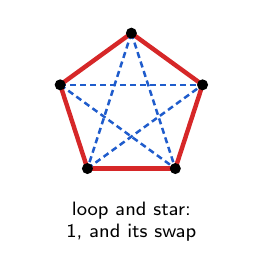
\begin{tikzpicture}[baseline=(current bounding box.north)]\draw[cred, line width=1.6pt] (0.000,0.950) -- (-0.904,0.294);
\draw[cblue, line width=0.9pt, dash pattern=on 2.2pt off 1.4pt] (0.000,0.950) -- (-0.558,-0.769);
\draw[cblue, line width=0.9pt, dash pattern=on 2.2pt off 1.4pt] (0.000,0.950) -- (0.558,-0.769);
\draw[cred, line width=1.6pt] (0.000,0.950) -- (0.904,0.294);
\draw[cred, line width=1.6pt] (-0.904,0.294) -- (-0.558,-0.769);
\draw[cblue, line width=0.9pt, dash pattern=on 2.2pt off 1.4pt] (-0.904,0.294) -- (0.558,-0.769);
\draw[cblue, line width=0.9pt, dash pattern=on 2.2pt off 1.4pt] (-0.904,0.294) -- (0.904,0.294);
\draw[cred, line width=1.6pt] (-0.558,-0.769) -- (0.558,-0.769);
\draw[cblue, line width=0.9pt, dash pattern=on 2.2pt off 1.4pt] (-0.558,-0.769) -- (0.904,0.294);
\draw[cred, line width=1.6pt] (0.558,-0.769) -- (0.904,0.294);
\fill (0.000,0.950) circle (0.07);
\fill (-0.904,0.294) circle (0.07);
\fill (-0.558,-0.769) circle (0.07);
\fill (0.558,-0.769) circle (0.07);
\fill (0.904,0.294) circle (0.07);
\node[font=\scriptsize, anchor=north, text width=2.4cm, align=center] at (0,-1.070) {loop and star: 1, and its swap};\end{tikzpicture}\hspace{0.3cm}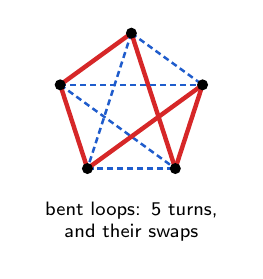
\begin{tikzpicture}[baseline=(current bounding box.north)]\draw[cred, line width=1.6pt] (0.000,0.950) -- (-0.904,0.294);
\draw[cblue, line width=0.9pt, dash pattern=on 2.2pt off 1.4pt] (0.000,0.950) -- (-0.558,-0.769);
\draw[cred, line width=1.6pt] (0.000,0.950) -- (0.558,-0.769);
\draw[cblue, line width=0.9pt, dash pattern=on 2.2pt off 1.4pt] (0.000,0.950) -- (0.904,0.294);
\draw[cred, line width=1.6pt] (-0.904,0.294) -- (-0.558,-0.769);
\draw[cblue, line width=0.9pt, dash pattern=on 2.2pt off 1.4pt] (-0.904,0.294) -- (0.558,-0.769);
\draw[cblue, line width=0.9pt, dash pattern=on 2.2pt off 1.4pt] (-0.904,0.294) -- (0.904,0.294);
\draw[cblue, line width=0.9pt, dash pattern=on 2.2pt off 1.4pt] (-0.558,-0.769) -- (0.558,-0.769);
\draw[cred, line width=1.6pt] (-0.558,-0.769) -- (0.904,0.294);
\draw[cred, line width=1.6pt] (0.558,-0.769) -- (0.904,0.294);
\fill (0.000,0.950) circle (0.07);
\fill (-0.904,0.294) circle (0.07);
\fill (-0.558,-0.769) circle (0.07);
\fill (0.558,-0.769) circle (0.07);
\fill (0.904,0.294) circle (0.07);
\node[font=\scriptsize, anchor=north, text width=2.4cm, align=center] at (0,-1.070) {bent loops: 5 turns, and their swaps};\end{tikzpicture}}
\newcommand{\sixfig}{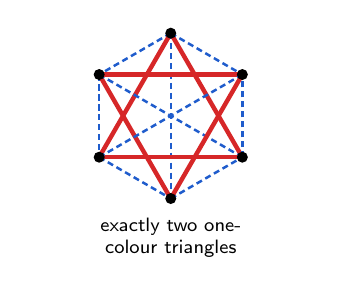
\begin{tikzpicture}[baseline=(current bounding box.north)]\draw[cblue, line width=0.9pt, dash pattern=on 2.2pt off 1.4pt] (0.000,1.050) -- (-0.909,0.525);
\draw[cred, line width=1.6pt] (0.000,1.050) -- (-0.909,-0.525);
\draw[cblue, line width=0.9pt, dash pattern=on 2.2pt off 1.4pt] (0.000,1.050) -- (-0.000,-1.050);
\draw[cred, line width=1.6pt] (0.000,1.050) -- (0.909,-0.525);
\draw[cblue, line width=0.9pt, dash pattern=on 2.2pt off 1.4pt] (0.000,1.050) -- (0.909,0.525);
\draw[cblue, line width=0.9pt, dash pattern=on 2.2pt off 1.4pt] (-0.909,0.525) -- (-0.909,-0.525);
\draw[cred, line width=1.6pt] (-0.909,0.525) -- (-0.000,-1.050);
\draw[cblue, line width=0.9pt, dash pattern=on 2.2pt off 1.4pt] (-0.909,0.525) -- (0.909,-0.525);
\draw[cred, line width=1.6pt] (-0.909,0.525) -- (0.909,0.525);
\draw[cblue, line width=0.9pt, dash pattern=on 2.2pt off 1.4pt] (-0.909,-0.525) -- (-0.000,-1.050);
\draw[cred, line width=1.6pt] (-0.909,-0.525) -- (0.909,-0.525);
\draw[cblue, line width=0.9pt, dash pattern=on 2.2pt off 1.4pt] (-0.909,-0.525) -- (0.909,0.525);
\draw[cblue, line width=0.9pt, dash pattern=on 2.2pt off 1.4pt] (-0.000,-1.050) -- (0.909,-0.525);
\draw[cred, line width=1.6pt] (-0.000,-1.050) -- (0.909,0.525);
\draw[cblue, line width=0.9pt, dash pattern=on 2.2pt off 1.4pt] (0.909,-0.525) -- (0.909,0.525);
\fill (0.000,1.050) circle (0.07);
\fill (-0.909,0.525) circle (0.07);
\fill (-0.909,-0.525) circle (0.07);
\fill (-0.000,-1.050) circle (0.07);
\fill (0.909,-0.525) circle (0.07);
\fill (0.909,0.525) circle (0.07);
\node[font=\scriptsize, anchor=north, text width=3.4cm, align=center] at (0,-1.170) {exactly two one-colour triangles};\end{tikzpicture}}

\begin{document}
\head{Mathematical overview: past a size, the pattern cannot be avoided}
Three times, children colour a set red or blue while avoiding a one-colour pattern. Each time a set of one size can avoid it and the next size cannot: every colouring contains the pattern. Every count below is computer-checked against the final pages.

\textbf{Equally spaced threes (van der Waerden number $W(3;2)=9$).} Colour squares $1,\dots,n$ red or blue. \emph{Equally spaced} means $a,\,a+d,\,a+2d$ for any $d\ge1$, so neighbours such as 4, 5, 6 count. Eight squares can avoid a one-colour three in exactly six ways: \st{RRBBRRBB}, \st{RBRBBRBR}, \st{RBBRRBBR} and their colour swaps. Nine squares cannot, so no longer strip can either (its first nine squares would be good). For $n=3,\dots,9$ the numbers of good strips are 6, 10, 14, 20, 16, 6, 0 (computer). \emph{Proof for nine.} If squares 4 and 6 match, say red, then 5, 2 and 8 must all be blue (because of $4,5,6$; $2,4,6$; $4,6,8$), and $2,5,8$ is equally spaced. If 4 and 6 differ, square 5 matches one of them; reversing the strip ($i\mapsto 10-i$ fixes 5 and swaps 4 with 6) and swapping colours, take 4 and 5 red, 6 blue. Then 3 is blue ($3,4,5$), 9 red ($3,6,9$), 7 blue ($5,7,9$), 8 red ($6,7,8$), 1 blue ($1,5,9$), and square 2 can be neither colour: red completes $2,5,8$, blue completes $1,2,3$. A second proof extends each good 8-strip (Grades 2--3 Problem 3). Combs 1--4 (Comb $d$ shows three squares $d$ apart) see all 16 equally spaced threes on nine squares.

\textbf{Sums (Schur).} Colour $1,\dots,n$ so that no $x+y=z$ has all three numbers one colour, where $x=y$ is allowed ($2+2=4$ counts). With two colours, $1,\dots,4$ works only as \st{RBBR} or \st{BRRB}, and $1,\dots,5$ never works: if 1 is red, then 2 is blue ($1+1$), 4 red ($2+2$), 3 blue ($1+3$), and 5 can be neither ($1+4$, $2+3$). With three colours, $1,\dots,13$ works and $1,\dots,14$ does not (computer search). Every good colouring of $1,\dots,13$ gives $\{1,4,10,13\}$, $\{2,3,11,12\}$ and $\{5,6,8,9\}$ three different colours, and 7 may take any colour: $3\times 6=18$ colourings. The convention changes the answer: if a number may not be added to itself (Grades 4--5 Problem 9), two colours reach 8, only as red $\{1,2,4,8\}$ and blue $\{3,5,6,7\}$ or the swap, and $1,\dots,9$ fails in three forced cases (given there).

\textbf{Triangles (Ramsey number $R(3,3)=6$).} Join every two of $n$ dots and colour each line red or blue. A \emph{one-colour triangle} is three dots joined by three lines of one colour; a crossing is not a dot. \emph{Six dots always have one.} A dot has five lines, so three of them share a colour, say red, going to $A$, $B$, $C$. A red line among $A$, $B$, $C$ closes a red triangle; if none is red, $A$, $B$, $C$ form a blue triangle. \emph{Five dots can avoid one}, in exactly 12 of the 1,024 colourings. A dot has four lines; three of one colour would force a triangle as above, so every dot has two red and two blue, and each colour forms one loop through all five dots. There are 12 loops through five labelled dots (choose dot 1's two neighbours in 6 ways; the loop goes round the other two dots in 2 orders). \emph{Six dots always have at least two} (Goodman 1959). Call a pair of lines at one dot a \emph{mixed corner} if their colours differ. A dot with $r$ red lines has $r(5-r)\le6$ mixed corners, so there are at most 36. A triangle that is not one colour has exactly two mixed corners and a one-colour triangle has none, so at most 18 of the 20 triangles are mixed. Two separate red triangles on alternate dots, with every other line blue, have exactly two. \emph{Sim} colours the six-dot board in turn, so it can never fill without a loser; the second player wins with perfect play (Mead, Rosa and Huang 1974, by computer; our check agrees), by no simple strategy we know.

\textbf{The general theorems behind the three thresholds.} Each threshold is the first case of a general theorem: for any number of colours and any length of pattern, a long enough strip, run of numbers or set of dots must contain it (van der Waerden 1927, Schur 1916, Ramsey 1930). The thresholds grow fast and are known only in small cases. Three colours need 27 squares to force a one-colour three; two colours need 35 squares to force four equally spaced squares of one colour; four colours need 45 numbers to force a one-colour sum (1 to 44 can be coloured); four dots with all six of their lines one colour need 18 dots, and for five dots the number is unknown. These are published results; we re-checked 27 and 35, and the colourings of 1 to 44 and of 17 dots, by computer. Children meet three first cases; the general theorems are adult background for the 4--5 question of how a threshold moves.

\textbf{Experiments, conjectures and explanations.} Many failed 9-strips support a conjecture; they do not explain it. The explanations here are \emph{forced chains}, where each colour decides the next until something can take neither colour (nine squares, five numbers, nine numbers without doubling), and \emph{pigeonhole} (six dots). A ``find every'' list is complete when its cases are organized, not when ideas run out. Game results (the strip game on nine, Sim) are computer facts; children can explain part: a full board holds the pattern, so if a game lasts that long, the last piece loses.

\textbf{What each band discovers.} \emph{K--1} (no reading when an adult reads; counting to 9; no arithmetic): build strips with counters, check with combs, finish strips whose squares are forced, find that 8 works and 9 does not, play the strip game and decide whether to go first. \emph{Grades 2--3} (short sentences; sums to 15): the same threshold with all six 8-strips and a case check for 9; sums up to 4 and 5; five dots; Sim; three colours. \emph{Grades 4--5} (sums to 15; written or spoken explanations): forced-chain proofs for nine squares and five numbers, all 12 five-dot colourings, the pigeonhole proof, the fewest triangles, and how the threshold moves when the rule changes (8 without doubling, 13 with three colours).

\head{Preparation, shared launch and pacing}
\textbf{Status.} Prepared for organizer review; unpiloted. Untested physically: counters and combs on the 25\,mm squares of the K--1 pages, especially a comb over a middle strip (it reaches 9\,mm above the strip it checks, 2\,mm short of the strip above on K--1 page 1, and covers that strip's numbers); whether the card combs' 6\,mm end posts stay stiff; colouring the faint lines of small dot boards (the 16 five-dot boards of Grades 4--5 page 4 are 3.9\,cm across); and every time estimate here.

\textbf{Print.} US Letter, single-sided, at 100\% (Actual size). One packet per child: K--1 has 6 landscape pages, Grades 2--3 has 6, Grades 4--5 has 7. Every K--1 strip has 25\,mm squares, so the K--1 pages are the working mats for counters and combs. The older packets' strips (15, 13 and 11\,mm squares) and number circles are for recording; older pairs build with counters on the materials file, \texttt{materials.pdf} (4 pages). Counts are for the current five pairs (two at K--1, two at 2--3, one at 4--5).

{\small\begin{tabular}{@{}>{\raggedright\arraybackslash}p{.06\linewidth}>{\raggedright\arraybackslash}p{.30\linewidth}>{\raggedright\arraybackslash}p{.26\linewidth}>{\raggedright\arraybackslash}p{.30\linewidth}@{}}\toprule
Page & Object & Print & Used in\\\midrule
1 & Combs 1--4 (34\,mm card, 23\,mm windows; cut out) & 5 on card stock, one set per pair; the launch borrows one & every K--1 problem; older Problems 1--3 on Materials page 2\\
2 & Strips of 6, 7, 8 and 9 squares (25\,mm) & 3, one per older pair & Grades 2--3 and 4--5 Problems 1--3\\
3 & Cards 1 to 15 (cut apart) and the launch strip of 5 squares & 3, on card if available, one per older pair & Grades 2--3 Problems 4, 5, 8; Grades 4--5 Problems 4, 9, 10; the launch\\
4 & Boards of six dots (12\,cm, two per sheet) & 7: two per older pair, one for K--1 Sim & Sim (2--3 Problem 7, 4--5 Problem 6); spare tries for 4--5 Problems 7--8\\\bottomrule
\end{tabular}}

\textbf{Per pair.} Red and blue counters no wider than 22\,mm (they then sit inside the 23\,mm comb windows and the 26\,mm card circles), 10 of each; add 6 green for the older pairs (no colour of a good colouring of $1,\dots,13$ has more than 5 numbers). K--1 pairs: red and blue crayons. Older pairs: red, blue and green coloured pencils and an ordinary pencil; children may write R, B or G in pencil while experimenting and colour only what they keep, since coloured pencil does not erase. A sheet protector over a dot board with dry-erase markers may also serve for Sim (untested).

\textbf{Preparation time.} About 50 minutes the first time: 10 to print (the comb sheets on card), 20--25 to cut the five comb sheets (about 5 minutes a sheet with scissors; a craft knife speeds the notches), 10 to cut the three card sheets and one launch strip, and 10 to count counters into five bags. Combs, cards, strips and counters are reusable, so a return visit needs only packets and fresh dot boards (about 10 minutes). These are estimates, not timed.

\textbf{Staffing.} One adult per table. The parent volunteer at K--1 reads each problem, plays the strip game against the children, and makes sure the combs are slid to every place after every turn; the children choose every colour. The Grades 2--3 adult reads the sum rule and the Sim rules and shows on a scrap drawing what counts as a triangle. At Grades 4--5 the third child referees: checks each strip or game move with the combs, or each colouring of numbers by its sums. Reading or recording for a child is ordinary help; choosing colours for a child means the task is too big, so return to a shorter strip.

\textbf{Launch after the run (about 4 minutes).} Hand out counters and combs for a minute. Then gather at the board, where everyone can see: draw five large numbered squares and use red and blue magnets or chalk circles. To show a comb, cover the squares it hides with sheets of paper (for Comb 2 at 1, 3, 5, cover squares 2 and 4). Once, lay the real Comb 1 over the printed launch strip (Materials page 3) and hold it up, so children see how a comb sits on a strip. No packet has a strip of five.
\begin{center}\launchfig\end{center}
Ask a child for a first try; the figure shows one possible run. Slide Comb 1 to every place it fits, then Comb 2 (Combs 3 and 4 do not fit on five squares; on longer strips, every comb that fits must be slid to every place). When a comb shows three of one colour, ask which counter to change, and check again: in the run shown, fixing 3, 4, 5 makes 1, 2, 3 all red, so fixing one three can make another. If a first try alternates colours, Comb 2 catches it at 1, 3, 5; use it, but do not suggest it. End with a strip the children propose that passes every comb position, such as \st{RRBRR}, which lies inside no good 8-strip. Say: ``A strip is good when no comb, anywhere, shows three counters of one colour.'' Say nothing about longer strips. For the older tables add one sentence: the comb windows are the equally spaced squares of their rule, as in their page 1 picture (a comb over 2, 5, 8). Sums and triangles get a one-minute demonstration when a table reaches them, again on non-task instances: cards 3, 4 and 7 all red break the rule ($3+4=7$), and so do 5 and 10 both red ($5+5=10$); on four dots with all six lines drawn, three dots joined by three red lines are a triangle, and the crossing in the middle is not a dot.

\textbf{A first visit.} After the run and launch, allow 35--40 minutes at tables and 5 for sharing. First routes: K--1 Problems 1--3, then the game of Problem 4 (one pair against the adult, the other pair against each other), ending the games with Problem 5's question asked aloud: ``On 9 squares, would you rather go first or second?'' Grades 2--3 Problems 1--3, with pairs pooling the six 8-strips in Problem 2, and Problems 4--5 if there is time. Grades 4--5 Problems 1--4, starting Problem 5 if there is time. Share one good 8-strip and what happened at 9, and one explanation. \textbf{Return visit:} K--1 Problem 5's game on 8 squares and Problem 6, then, optionally and untested, Sim against the adult on a board from Materials page 4: no reading is needed, the adult checks each new line for a triangle, and a child shows one with three fingers on its three dots. Grades 2--3 Problems 6--8; Grades 4--5 Problems 5--8, with 9--10 as a continuation. Finishing every page is not the goal.

\textbf{Watch for.} Each is a likely slip, not an observation. A comb slid to only some places (``wherever you slide it''). Older children forgetting neighbours (Comb 1) or Combs 3 and 4. Forgetting doubles ($2+2=4$) in the sums. Counting the small triangles made by crossing lines in Sim.

\head{Grades K--1: a plain-words key}
Every strip on these pages has 25\,mm squares: counters go on the page and Combs 1--4 (Materials page 1) slide over them; a comb's number is how far apart its windows are. Lay a comb with its tooth ends on the strip's bottom edge, so the numbers under the strip stay visible. Where a page says colour, a crayon dot in each square is enough. Letters below are colours read from square 1: \st{R} red, \st{B} blue. The half-size picture on page 1 shows a full strip with Comb 2 at 2, 4, 6 finding three reds (blue 3 and 5 are under the card).

\sub{Problem 1, page 1: strips of 4, 6 and 7}
All three can be made good, in 10, 20 and 16 ways. Examples: \st{RRBB}, \st{RRBBRR}, \st{RRBBRRB}. To check a child's strip, slide every comb to every place it fits. Taking turns with colours works on 4 squares, but on 6 and 7 Comb 2 at 1, 3, 5 shows three reds. Hint, only if needed: ``Which comb found the problem? Which counter could you change?''

\sub{Problem 2, page 2: finish each strip}
Each strip has exactly one answer:
\st{BRRBBRR} (7 squares, red at 2 and 3); \st{RRBBRRBB}; \st{RBRBBRBR}; \st{RBBRRBBR}. A strip that differs from these will show three of one colour under some comb. The 7-strip goes square by square: 1 and 4 must be blue (else three reds), then 7 red (1, 4, 7), 5 blue (3, 5, 7), 6 red (4, 5, 6). Each 8-strip has one or two forced squares and then needs one try. The second strip is the \st{RR} start under Problem 6. On the third, 3 and 6 must be red, and square 1 must be red. On the fourth, 2 must be blue and square 1 must be red. Hints: ``Is there a square that can only be one colour?'' ``If you try red here, what happens next?'' The three 8-strips are three of the six answers to Problem 6.

\sub{Problem 3, page 3: 8 squares, then 9}
Eight: yes, six ways (Problem 6); the 8-strips from Problem 2 work. Nine: no strip of 9 can be good. Children may conclude this from many tries (``when we fix one, another breaks''). If a child shows a good-looking 9-strip, slide all four combs along it with the child: some comb shows three of one colour. ``How do you know for sure?'' for a ready child: put a ninth square on each good 8-strip and try both colours; the combs catch every one. The full proof is in the overview.

\sub{Problem 4, page 4: the game on 9 squares}
Either player may use either colour on any turn; say so, since a child may assume one colour each. Because no 9-strip is good, every game has a loser. Only threes through the newest counter can be new, so slide each comb to the places where one window covers that counter. With perfect play the second player wins (computer), by no simple rule we know. With both players choosing safe moves at random, the first player loses a little over half the games, almost always on the ninth counter; otherwise the second player is stuck on the eighth. Make real safe moves, do not throw games, and let children go first and second.

\sub{Problem 5, page 4: the game on 8 squares; first or second on 9}
On 8 squares a game can end full with nobody losing: the final strip is one of the six good 8-strips, and with best play by both nobody loses (computer). Random safe play fills the strip only about one game in five, so children may first answer no; ask ``Can you two fill it together with nobody losing?'' On 9 squares, the reason to want to go second: if all the other squares fill safely, the ninth counter must make three of one colour, and the first player places counters 1, 3, 5, 7 and 9. Games often end at the eighth counter instead, so accept any answer with a reason; this one is the prize.

\sub{Problem 6, pages 5--6: every good strip of 8}
Six: \st{RRBBRRBB}, \st{RBRBBRBR}, \st{RBBRRBBR}, and the same with colours swapped (\st{BBRRBBRR}, \st{BRBRRBRB}, \st{BRRBBRRB}). The pages give exactly six strips, so a child who fills them all correctly is done. Ten counters of each colour hold only two 8-strips at once, so when a strip passes every comb, the children dot each square in crayon and move the counters to the next strip. Why there are no more: a strip starting red begins \st{RR}, \st{RBR} or \st{RBB}, and each start allows only one good 8-strip, found with at most one try.
\begin{itemize}[leftmargin=1.2em]
\item \st{RR}: 3 must be blue. If 4 is red, then 6 and 7 are blue (2, 4, 6; 1, 4, 7), 5 is red (5, 6, 7), and 8 can be neither (2, 5, 8; 6, 7, 8). So 4 is blue, and the rest is forced: \st{RRBBRRBB}.
\item \st{RBR}: 5 must be blue (1, 3, 5) and 8 red (2, 5, 8). If 4 is red, 6 is blue (4, 6, 8), and 7 can be neither (1, 4, 7; 5, 6, 7). So 4 is blue, and the rest is forced: \st{RBRBBRBR}.
\item \st{RBB}: every square is forced: 4 red (2, 3, 4), 7 blue (1, 4, 7), 5 red (3, 5, 7), 6 blue (4, 5, 6), 8 red (6, 7, 8): \st{RBBRRBBR}.
\end{itemize}
Swapping colours gives the three starting blue. Turning a strip end to end gives nothing new: the first reversed is the colour swap of itself, and the other two read the same both ways. Hint: ``Can you make a new good strip from one you already have?''

\head{Grades 2--3}
Pairs build with counters on the 25\,mm strips of Materials page 2 and check with the combs, then colour what they keep on their own pages. The cards of Materials page 3 carry counters for Problems 4, 5 and 8.

\sub{Problem 1, page 1: the longest good strip}
Eight. Strips of 6, 7 and 8 can be good; the 9-strip cannot (Problem 3). Children who reach 8 may record any of the six. Hint: ``Which combs fit on this strip, and did you check them all?''

\sub{Problem 2, page 2: every good 8-strip}
The six listed under K--1 Problem 6; the page has eight strips, two spare. Pairs can share the search and pool a checked list. Completeness: the starts \st{RR}, \st{RBR}, \st{RBB} and their swaps each allow exactly one strip (the three short cases under K--1 Problem 6). Hint: ``If square 1 is red, what can squares 2 and 3 be?''

\sub{Problem 3, page 3: can 9 squares be good?}
No. The explanation within reach uses Problem 2's complete list: the first eight squares of a good 9-strip would form a good 8-strip, and each fails at square 9 in both colours. With square 9 red or blue, \st{RRBBRRBB} completes 1, 5, 9 or 7, 8, 9; \st{RBRBBRBR} completes 3, 6, 9 or 5, 7, 9; \st{RBBRRBBR} completes 1, 5, 9 or 3, 6, 9. The colour swaps fail at the same squares with the colours exchanged. The argument is only as good as the list, so ask: ``How do you know your list of good 8-strips is complete?'' Children ready for more can try the forced chain from the middle squares in the overview. Extension: ``Can a strip of 10 be good?'' (No: its first nine squares would be.)

\sub{Problem 4, page 4: cards 1 to 4}
Two ways: \st{RBBR} and \st{BRRB} (1 and 4 one colour, 2 and 3 the other). If 1 is red, then 2 is blue ($1+1=2$), 4 is red ($2+2=4$) and 3 is blue ($1+3=4$); the check $1+2=3$ passes. Starting with blue gives the swap. Hint: ``If card 1 is red, what can card 2 be?''

\sub{Problem 5, page 4: cards 1 to 5}
No. Cards 1 to 4 must be coloured as in Problem 4. Then $1+4=5$ (1 and 4 match) forbids one colour for 5, and $2+3=5$ (2 and 3 match) forbids the other. Hint: ``Which two cards add up to 5?''

\sub{Problem 6, page 5: five dots}
Possible, for example the five outside lines red and the five inside lines (the star) blue. There are 12 good colourings; see Grades 4--5 Problem 5. To show a triangle, a child puts three fingers on its three dots. Hint: ``Look at one dot. What colours are its four lines?'' Extension: find a good colouring that is not an outside loop and a star.

\sub{Problem 7, page 6: Sim}
Play on the page or on the larger boards of Materials page 4. No game can end with all fifteen lines coloured and nobody losing: every colouring of the six-dot board has a one-colour triangle, and a triangle in your own colour loses. The first player colours lines 1, 3, \dots, 15, so if no one has lost after fourteen lines, the first player loses on the last one. At 2--3 this is a conjecture from games; with a ready child, try the pigeonhole argument at one dot (overview).

\sub{Problem 8, page 6: three colours}
Thirteen. Every good colouring of 1 to 13 colours $\{1,4,10,13\}$, $\{2,3,11,12\}$ and $\{5,6,8,9\}$ in three different colours, and 7 may be any colour. Fourteen is impossible (computer). Colouring in order without going back usually stops early (always taking the first colour allowed stops at 7; with 1 red, only 6 of the 278 dead ends reach 13), so reaching 13 usually needs going back. Hints: ``Could your cards from Problem 4 help?'' (\st{RBBR} at 1--4, again at 10--13, green between.) ``Which numbers could all be green together?'' Extension: ``Why can 7 be any colour?''

\head{Grades 4--5}
Materials as for Grades 2--3: page 2 strips for Problems 1--3, page 3 cards for Problems 4, 9 and 10, and page 4 boards for Sim and spare tries.

\sub{Problems 1--2, pages 1--2: the longest strip and all its colourings}
Eight; six colourings, as for Grades 2--3 (page 2 has eight strips for six answers; completeness under K--1 Problem 6).

\sub{Problem 3, page 3: can 9 squares be good?}
No. Expect either the extension check (Grades 2--3 Problem 3), which rests on a complete list, or the forced chain in the overview, which does not. Hints, in order: ``Pick a square near the middle. What does its colour force?'' ``What if squares 4 and 6 are the same colour?'' The step ``reverse the strip and swap colours'' is the hardest; a child may instead do both cases by hand. With 4 red and 6 blue, if 5 is red the chain is the overview's; if 5 is blue, then 7 is red (5, 6, 7), 1 blue (1, 4, 7), 3 red (1, 3, 5), 2 blue (2, 3, 4) and 9 red (1, 5, 9), and 8 can be neither colour (7, 8, 9 would be all red; 2, 5, 8 all blue). With 4 blue, swap the colours.

\sub{Problem 4, page 3: two colours, doubling counts}
Four, only \st{RBBR} or \st{BRRB}; no colouring reaches 5 (chain under Grades 2--3 Problems 4--5). A child who colours 1, 2, 3 as \st{RBR} is stuck at 3: $2+2=4$ wants 4 red and $1+3=4$ wants it blue. That is a dead end, not the limit; ask, ``Is that as far as anyone can go, or as far as this colouring goes?'' A complete answer to ``why no colouring can go further'' starts from 1 and shows every choice is forced.

\needspace{11\baselineskip}\begin{minipage}[t]{.62\linewidth}
\sub{Problem 5, page 4: every way for five dots}
Twelve on labelled dots, of two shapes (right). The red outside loop with the blue star and its swap give 2; the bent loop (three outside lines and two crossing diagonals in one colour, the remaining two outside lines and three diagonals in the other) gives 5 turns and their swaps, 10. The page has 16 boards. Completeness is the loop argument in the overview; counting the red outside lines also sorts them: 5, 0, 3 or 2 give 1, 1, 5 and 5 colourings. A child who counts turned copies as the same finds 4, and 2 if swapped colours also count as the same (flips add nothing); ask what they count as different, and accept 12, 4 or 2 to match. Hint: ``Could three lines at one dot be red?''
\end{minipage}\hfill
\begin{minipage}[t]{.35\linewidth}\vspace{6pt}\centering\fivefig\end{minipage}\par\smallskip

\sub{Problem 6, page 5: Sim, first or second?}
Second: the second player wins with perfect play (computer). The part children can explain is the last-line argument under Grades 2--3 Problem 7. Games usually end sooner, and no simple strategy is known to us, so accept ``second'' with this reason, or a reasoned ``it depends''. Rotate the referee, who checks each new line for a triangle of the mover's colour.

\sub{Problem 7, page 5: six dots}
No colouring avoids a one-colour triangle; the pigeonhole proof is in the overview. A child's version: ``This dot has five lines, so three are the same colour, red, going to $A$, $B$ and $C$. If any line between $A$, $B$, $C$ is red, that makes a red triangle. If not, they are all blue: a blue triangle.'' Hints: ``Look at one dot's five lines. What must be true about their colours?'' ``Three red lines go to $A$, $B$, $C$. What about the lines between them?'' Ask why the same argument does not work for five dots (Problem 5).

\needspace{11\baselineskip}\begin{minipage}[t]{.70\linewidth}
\sub{Problem 8, page 6: as few triangles as possible}
Two. Example: red on the two big triangles of the six-pointed star (alternate dots), blue elsewhere. Any three dots include two from the same red triangle, joined in red, so there is no blue triangle. Exactly 1,760 of the 32,768 colourings have two, and none has fewer. The mixed-corner count in the overview proves ``at least two'' and is a good conversation at this table once children believe 2 is the minimum. Extension: can you get exactly 3? (Yes.) For the referee: at each dot, for each pair of same-colour lines, check the line joining their ends; each one-colour triangle turns up once at each of its three corners, so divide the total by 3.
\end{minipage}\hfill
\begin{minipage}[t]{.26\linewidth}\vspace{4pt}\centering\sixfig\end{minipage}\par\smallskip

\sub{Problem 9, page 7: no doubling}
Eight, only red $\{1,2,4,8\}$, blue $\{3,5,6,7\}$ (\st{RRBRBBBR}) or the swap. Now 1 and 2 may match. Why 9 fails, taking 1 red: if 3 is red, then 2 blue ($1+2$), 4 blue ($1+3$), 6 red ($2+4$), 9 blue ($3+6$), 5 red ($4+5$), and $1+5=6$ is all red. If 3 is blue and 4 red, then 5 blue ($1+4$), 2 red ($2+3$), 6 blue ($2+4$), 8 red ($3+5$), 9 red ($3+6$), and $1+8=9$ is all red. If 3 and 4 are blue, then 7 red ($3+4$), 6 blue ($1+6$), 8 blue ($1+7$), 2 red ($2+4$), 5 blue ($2+5$), and $3+5=8$ is all blue. Hint: ``What does $1+2=3$ say about 3 now?''

\sub{Problem 10, page 7: three colours}
Thirteen, with the structure given under Grades 2--3 Problem 8; fourteen is impossible (computer). Building on Problem 4 (\st{RBBR} at both ends, a third colour for 5--9) is the natural route.

\head{Sources, connections and what to record}
None of the outline's references was available in this checkout, so none was read for this guide; every fact above is computer-checked against the final pages, and the hand proofs are our own. References from the outline: R.\,L. Graham, B.\,L. Rothschild and J.\,H. Spencer, \emph{Ramsey Theory}, 2nd ed., Wiley 1990, chapters 1--2 (sections not checked); B.\,L. van der Waerden, Nieuw Archief voor Wiskunde 15 (1927); I. Schur, Jahresbericht der DMV 25 (1916); R.\,E. Greenwood and A.\,M. Gleason, Canadian Journal of Mathematics 7 (1955); A.\,W. Goodman, American Mathematical Monthly 66 (1959); G.\,J. Simmons, ``The game of SIM'', Journal of Recreational Mathematics 2 (1969); E. Mead, A. Rosa and C. Huang (1974), Sim by computer; New York Times Numberplay, ``Don't Make a Triangle'', Parts 1 and 2 (local copies are not in this checkout). Cited for the general theorems, also not consulted: F.\,P. Ramsey, Proceedings of the London Mathematical Society 30 (1930); V. Chv\'atal (1970) for 27 and 35; L.\,D. Baumert (1965) for 44. Related references listed in the repository's resource manifest, not in this checkout and not consulted: Julia Robinson Mathematics Festival, ``Color Triangles''; Early Family Math, ``K--3 Sim Triangle''. Library: Week 36 (Making threes) seeks the largest set with no three and its return visit colours tiles in a Ramsey style; Week 55 (Few sums and equal spacing) adds sets of numbers; Week 62 colours conflict networks. New here: the threshold where avoiding becomes impossible, met three times, with pigeonhole as a proof. Record which problems each child reached, explanations in their words, whether the combs were used without prompting and lay flat over the K--1 strips, and the real preparation time.
\end{document}
